\chapter{Results}%
\label{chap:results}
\textit{This chapter presents the test results that test and challenge the proposed framework.  The randomization tests, which additionally test the influence of the \ac{kgraph} and test taken including and excluding the \ac{kgraph}. The test results provide evidence that supports the effectiveness of the proposed framework. This chapter starts by introducing \textbf{method metrics} that indicate how a task has been executed by the proposed framework in \Cref{sec:proposed_method_metrics}. A comparison is made with the state-of-the-art methods in \Cref{sec:compare_with_related_papers}. \bs}

\paragraph{The Simulation Environment}
Testing in a simulation environment has been done using the URDF Gym Environment~\cite{spahn_urdfenvironment_2022}, a 100\% python environment build upon the PyBullet library~\cite{coumans_pybullet_2016}. The code created during the thesis can be found on \href{https://gitlab.tudelft.nl/airlab-delft/msc_projects/msc_gijs_groote}{GitLab} and \href{https://github.com/GijsGroote/semantic-thinking-robot}{GitHub}. Experiments ran on standard TU Delft laptop: HP ZBook Studio x360 G5, running OS:~Ubuntu 22.04.1 LTS x86\_64, CPU: Intel i7-8750H (12) @ 4.100GHz, GPU: NVIDIA Quadro P1000 Mobile.\bs
The simulation environment provides many different robots, of which two simple robots are selected to perform tests, they are displayed in \Cref{fig:example_robots}, and various objects are displayed in \Cref{fig:example_objects}.

\section{Proposed Method Metrics}%
\label{sec:proposed_method_metrics}
\todo{Corrado: I’m confused, what metric is exactly used? Write it explicitly, GIJS: first sentece here}
The results are measured in method metrics, not to be confused with the monitoring metrics in \Cref{sec:monitoring_metrics} or the edge metrics in \Cref{subsec:edge_metrics}. The results are interesting, but most interesting is the progression of the method metrics over time. As will be shown, the effect of learning can be measured by investigating and tracking the method metrics over time. Furthermore, the method metrics will be used to compare the proposed framework to relative state-of-the-art papers. First, the method metrics are presented in~\Cref{table:proposed_method_metrics} with corresponding argumentation on the relevance of the metric.\bs

\todo{Corrado: I’m very confused by what metric is used for what part and why some metric (from earlier) are not used but still presented }
\noindent
\begin{table}[H]
\centering
\begin{tabular}%
  {>{\raggedright\arraybackslash}p{0.25\textwidth}%
   >{\raggedright\arraybackslash}p{0.65\textwidth}}
Total Average\newline \acl{PE} & The total average \ac{PE} is calculated by augmenting every prediction error into a single list, then the mean and standart deviation are calculated over that list. Since the \ac{PE} is high when unexpected behaviour occurs, seeing the total average \ac{PE} lower would indicate the robot encounters less unexpected behaviour, indicating the robot is learning.\\
% Total Average\newline \acl{TE}& The total average \ac{TE} is created by averaging over every hypothesis' average \ac{TE} in a \ac{hgraph}. Seeing the total average \ac{TE} lower over time would indicate the robot is selecting better suitable controllers and system models, indicating the robot is learning.\\
% Final positions and\newline displacement errors & The final position and displacement error is a metric which how a controller performs. This thesis does not create or investigate controllers, but it is interesting to see why different controllers are preferred for different objects. The final position and displacement error could be the cause.\\
The ratio between the number of hypotheses and the number of tasks & Expected is that whilst learning system models, the hypothesis created will be more effective. Thus the ratio between the total number of hypotheses and the total number of tasks is expected to lower with new knowledge.\\
The ratio between the number of successful and the number of total edges in \ac{kgraph} & When the \ac{kgraph} improves recommending a controller and system model, the ratio between successful edges and total edges is expected to increase because, with better recommendations, more edges will be completed.\\
task completion time =\newline run time + planning time& If equal tasks are given multiple times, the total task completion time should drop pretty drastically. Multiple factors help to lower the task completion time, firstly system identification has to be performed only once, and there is no need to lose time on redoing system identification. Secondly, the \ac{hgraph} is expected to improve generated hypothesis, or better said, the same mistake should not be made multiple times, resulting in fewer failing hypotheses and lowering task completion time.\\
\end{tabular}
\caption{Proposed method metrics used to compare the proposed framework with the state-of-the-art.}\label{table:proposed_method_metrics}
\end{table}

Three system models are used for testing. The goal of this thesis is not to find optimal control, or to model the environment very accurately. The goal is to select the best combination of controller and system model in the available set of controllers and system models. Only a short textual description of the available system models is provided below.\bs


\todo{Martijn: you don't explain what these models are, nor do you re-use these model names anywhere in the thesis.}
\noindent
\begin{table}[H]
\centering
\begin{tabular}%
  {>{\raggedright\arraybackslash}p{0.25\textwidth}%
   >{\raggedright\arraybackslash}p{0.65\textwidth}}
\textit{lti-drive-model} & A second order \ac{LTI} model that can be used by both the \ac{MPC} and the \ac{MPPI} drive controller. The next robot configuration is based on the current configuration and system input in \gls{x} and \gls{y} direction. \\
\textit{nonlinear-push-model-1} & A nonlinear model describing the next object configuration in \gls{x} and \gls{y} direction and the orientation \gls{theta} based on the current configurations of the robot, the object and on the robot inputs in \gls{x} and \gls{y} direction.\\
\textit{nonlinear-push-model-2} & A nonlinear model describing the next object configuration in \gls{x} and \gls{y}, and the object configuration in \gls{x} and \gls{y} direction based on the current configurations of the robot, the object and on the robot inputs in \gls{x} and \gls{y} direction.\\
\end{tabular}
\caption{Available drive and push system models used for testing.}\label{table:available_system_models}
\end{table}
\todo{Corrado: Missing the details. You need to add these models in order for someone to be able to reproduce the results or at least understand them GIJS: Add the formula's for these models}


% \todo[inline]{make the environment that shows learning object is unmovable}
% \begin{figure}[H]
%     \centering
%     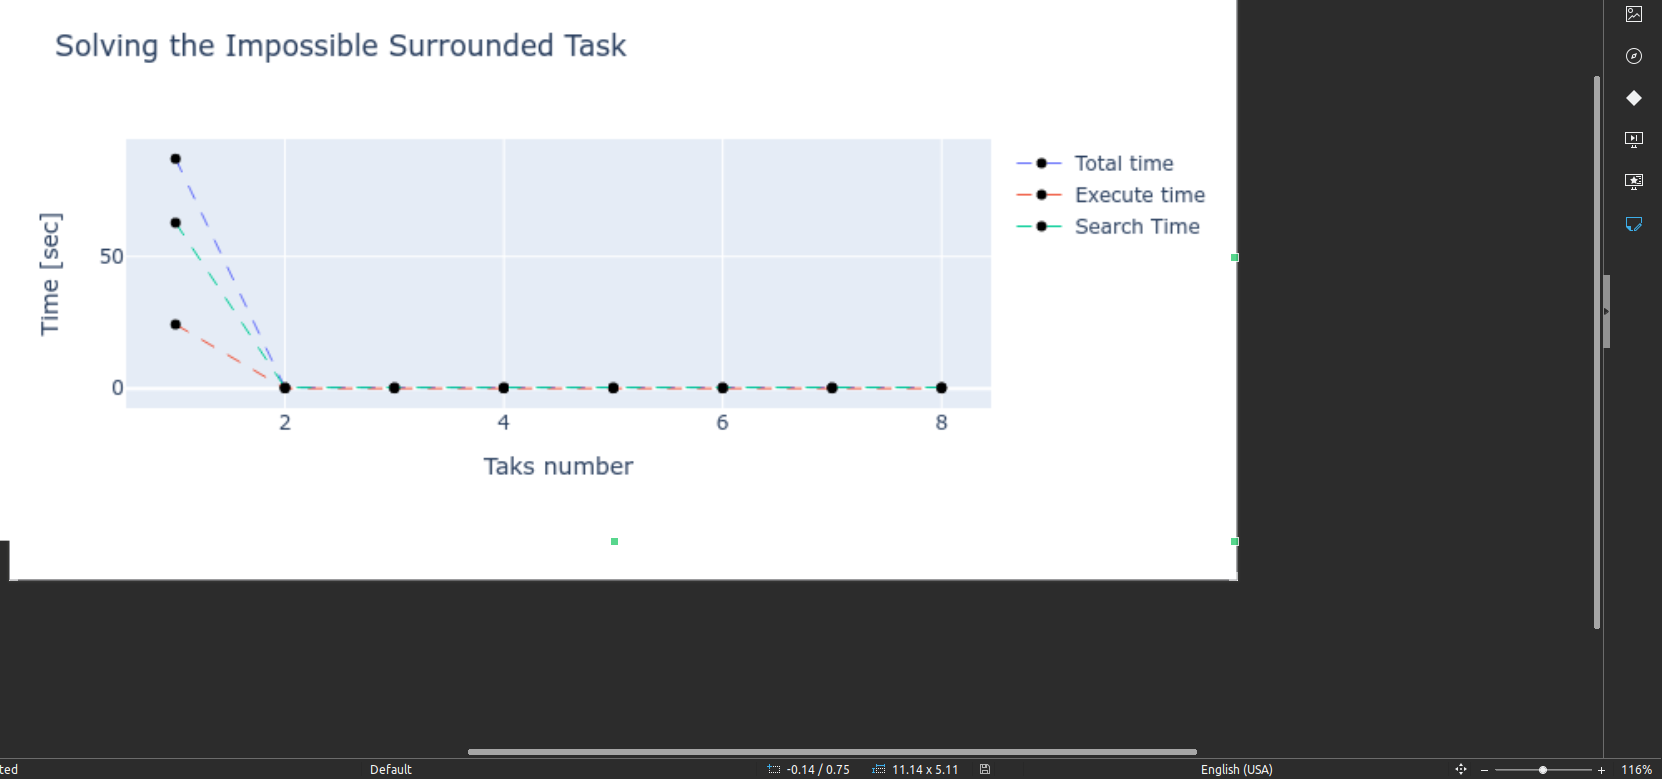
\includegraphics[width=5cm]{figures/results/execution_time_move_2}
% figures/figures/figures/figures/
%     \caption{}%
%     \label{}
% \end{figure}


% \section{Benchmark Tests}%
% \label{sec:benchmark_tests}
% Three benchmark test are presented, starting with the blockade task. A large part of the proposed framework is system identification, for testing however no system identification is performed. Instead, several hard-coded system models are used, and the \ac{kgraph} finds which system model is the best choice for an object over time. Where the best choice is defined using the edge metrics discussed in \Cref{subsec:edge_metrics}. The hard-coded system models are not opting for modelling the drive or push model as accurately as they possibly can, thus severe model mismatch should be expected. Such model mismatch is no issue, to complete a subtask stable closed-loop control is required, when an edge parameterization is unable to provide closed-loop stable control, the edge will fail because a fault will be detected. To answer the research question, improvement over time should be made. Gaining such improvement does not require accurate system models, time spend improving the hand-coded system models does thus not change the result.\bs
%
%
% \paragraph{Blockade} In the blockade environment the robot is tasked with placing a box in a target position that is blocked by a cylinder object.\bs
% \begin{figure}[H]
%     \centering
%     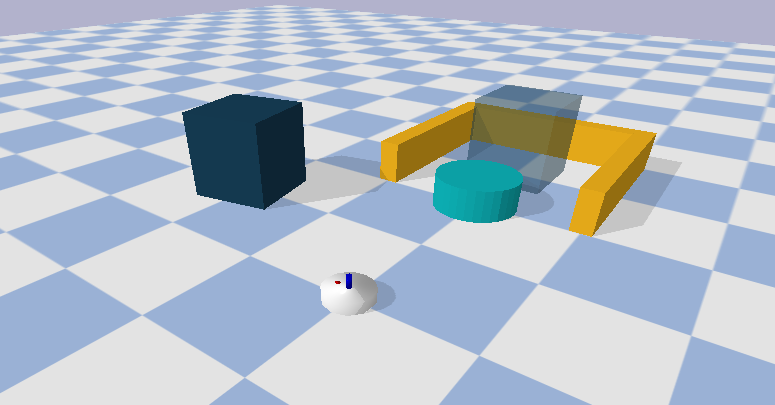
\includegraphics[width=0.9\textwidth]{figures/results/blockade}
%     \caption{The blockade environment with the target ghost position for the blue box. The green walls are unmovable whilst both the blue box and cylinder are movable.}%
%     \label{fig:benchmark_blockade}
% \end{figure}
%
% The blockade task neatly shows that the \ac{halgorithm} uses the backward search technique. First, the \ac{halgorithm} plans to push the box directly to the target position, then it realizes a blocking object must first be moved to free the path. It makes the mistake of pushing the unmovable wall, then it succeeds in pushing the movable cylinder out of the way. The \ac{kgraph} then ensures that this mistake will not occur again because is remembered that the wall is immovable. Over time the \ac{kgraph} indicates that it prefers to use the \ac{MPPI} controller with the nonlinear-push-model-2 to push both the box and the cylinder object. Converging to this conclusion improves the method metrics for the task as can be seen in \Cref{fig:results_blockade}\bs
%
% \todo[inline]{is nonlinear-push-model-2 still the preferred model after testing??}
%
% \begin{figure}[H]
%     \centering
%     
\includegraphics[width=0.9\textwidth]{figures/tests/404_not_found}
%
%     \caption{Some results are still under development for the blockade environment}%
%     \label{fig:results_blockade}
% \end{figure}
% \todo[inline]{Test to create results for running the blockade environment, and input into above 404 not found}
%
% \paragraph{Swap}
% In the swap environment the robot should swap the locations of the 2 objects in the environment.\bs
%
% \begin{figure}[H]
%     \centering
%     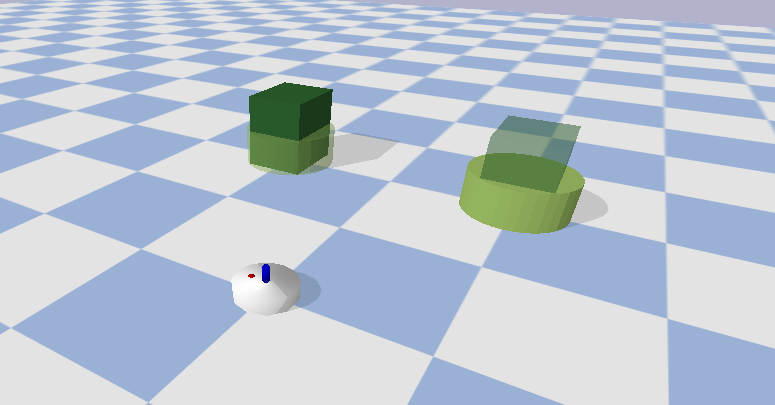
\includegraphics[width=0.9\textwidth]{figures/results/swap}
%     \caption{The swap environment, the robot is tasked with swapping the positions of the cylinder and the box.}%
%     \label{fig:benchmark_swap}
% \end{figure}
% The swap task shows that the \ac{halgorithm} can handle overlapping subtasks. The \ac{halgorithm} handles a single subtask at a time and randomly selects which subtask to handle next. The result for the swap task is that first, the robot will place the box on the location of the cylinder. The cylinder is blocking the path and is thus pushed to free the path, then the robot drives back to the box to push the box to its target position. The cylinder can directly be pushed toward its target position, because there is a free path, and the task is successfully completed. By manual inspection, this is the most efficient action sequence to complete the swap task. But there is an assumption because the initial environment has a distance between the robot and box (robot-box distance), and robot and cylinder (robot-cylinder distance) that is equal. If the initial robot-box distance is greater than the initial robot-cylinder distance, it would be more efficient to first drive toward the cylinder because that distance is smaller. The selection of subtask is random, thus there is a 50\% chance that the robot selects a subtask resulting in driving more than is necessary to complete the swap subtask.\bs
%
% \begin{figure}[H]
%     \centering
%     
\includegraphics[width=0.9\textwidth]{figures/results/404_not_found}
%     \caption{Some tests are still under development for the swap environment}%
%     \label{fig:results_swap}
% \end{figure}
%
% \todo[inline]{Test to create results for running the swap environment}
%
% \paragraph{Surrounded} In the surround environment the robot has to learn which box is movable to escape the enclosure of boxes.\bs
% \begin{figure}[H]
%     \centering
%     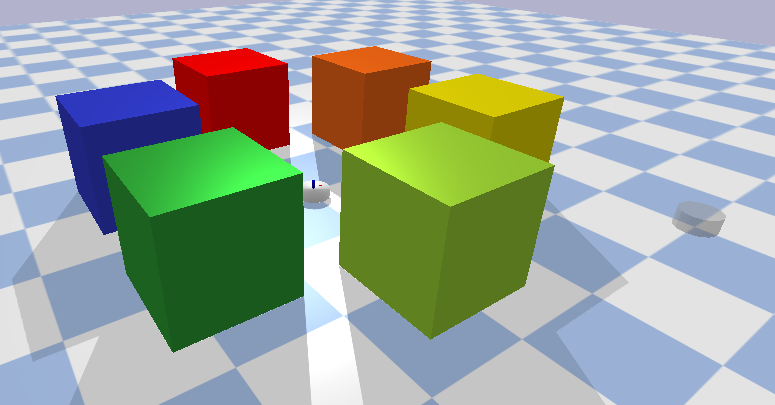
\includegraphics[width=0.9\textwidth]{figures/results/surrounded}
%     \caption{The surround environment, the robot is tasked with escaping the surrounding enclosure by driving to the target ghost position displayed on the right side in the figure. Every box objects is unmovable except the red box which is movable.}%
%     \label{fig:benchmark_surround}
% \end{figure}
% The surround task show that having and gaining environment knowledge can greatly improve task execution. Simply knowing if an object can be interacted with may lower task execution time drastically as can be seen in \Cref{fig:results_surround}.\bs
%
% \begin{figure}[H]
%     \centering
%     
\includegraphics[width=0.9\textwidth]{figures/results/404_not_found}
%     \caption{Some test are still under development for the surround environment}%
%     \label{fig:results_surround}
% \end{figure}
%
% \todo[inline]{Test to create results for running the surround environment}

\section{Randomization}%
\label{sec:randomisation}
The randomized environment ensures random objects at random initial poses within the specified ranges. These preconfigured ranges can be viewed in \Cref{table:configure_rand_env}. Two type of tasks are given to the robot to solve, an driving task, where the robot must drive toward a target pose, and a pushing task, where the robot must push an movable object toward a target pose. Performing tasks in a randomized environment produces unbiased results.\bs

\noindent
\begin{table}[H]
\centering
\begin{tabular}%
{>{\raggedright\arraybackslash}p{0.25\textwidth}%
>{\raggedright\arraybackslash}p{0.65\textwidth}}
The \textit{size of the grid} & length and width of the ground plane in \gls{x} and \gls{y} direction.\\
The \textit{minimal and maximal size of objects} & A box will have sides with a length that lie in the specified range from minimal to maximal length. Cylinders will have a diameter and height that is within the specified range, additionally, cylinders are not higher than the radius of the cylinder to prevent cylinders from tipping over. \\
The \textit{maximal weight} & which is uniformly distributed for the environment objects, minimal weight is set by default to 1 gram. \\
The \textit{number of unmovable objects} & Specify the amount of unmovable objects.\\
The \textit{number of movable objects} & Specify the amount of movable objects.\\
The \textit{number of subtasks in a task} & Specify the amount of subtasks in a task.
\end{tabular}
\caption{The tuning parameters that must be specified for the random environment}%
\label{table:configure_rand_env}
\end{table}

Lastly, the ratio between cylinders and boxes should be set. For every new object generated there is a 50\% chance it becomes a box and 50\% chance it becomes a cylinder, letting randomization determine the ratio between boxes and cylinders. \\

The environment can be \textit{reshuffled}, reshuffle the random environment does the following. First, the robots position is reset to the origin \gls{origin}, every object is set to a new initial position whilst their properties are unchanged. Lastly, objects that are in the task receive a new target pose. The objects in the task remain constant, whilst the target pose changes with every reshuffle. Solving multiple tasks in with reshuffles after task completion is named \textit{a run}, at the start of a run the \ac{kgraph} is empty, and at the end of a run the \ac{kgraph} is filled with the gained experience. The reshuffle functionality can be visualised in \Cref{fig:random_environment_reshuffle}. By solving a similar task in an reshuffled random environment multiple times, the robot gains experience and task exection can be investigated. With the investigation trends in task execution is monitored, to see improvement whilst gaining experience.\bs

\begin{figure}[H]
    \centering
    \begin{subfigure}{.49\textwidth}
    \centering
    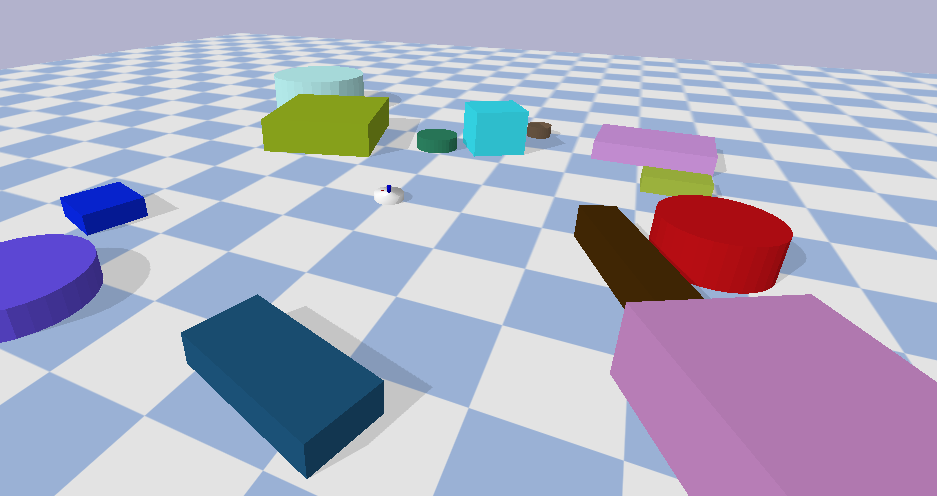
\includegraphics[width=\textwidth]{figures/results/random1}
    \end{subfigure}
    \hfill
    \begin{subfigure}{.49\textwidth}
    \centering
    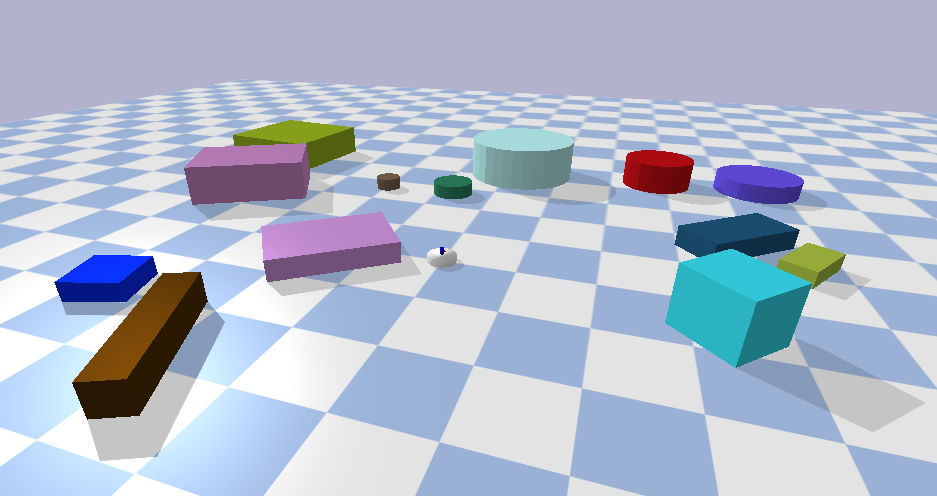
\includegraphics[width=\textwidth]{figures/results/random2}
    \end{subfigure}

    \vspace{0.2cm}
    \begin{subfigure}{.49\textwidth}
    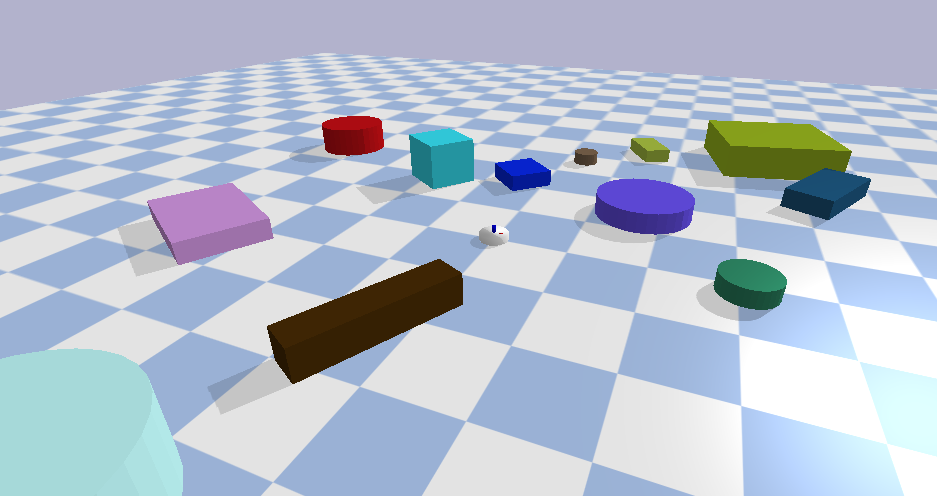
\includegraphics[width=\textwidth]{figures/results/random3}
    \end{subfigure}
    \hfill
    \begin{subfigure}{.49\textwidth}
    \centering
    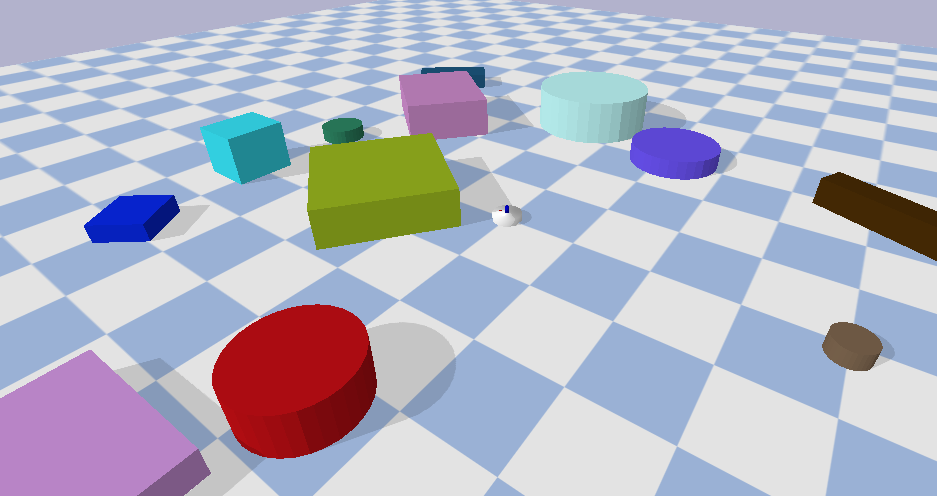
\includegraphics[width=\textwidth]{figures/results/random4}
    \end{subfigure}
    \caption{A random environment initialised by tuning parameters presented in \Cref{table:configure_rand_env_values}. After initialisation the environment is reshuffled three times}%
    \label{fig:random_environment_reshuffle}
\end{figure}

\subsection{A Driving Task}%
\label{subsec:rand_driving}
For the driving task the random environment is created with the following tuning parameters.\bs

\begin{table}[H]
\centering
\begin{tabular}%
{>{\raggedright\arraybackslash}p{0.25\textwidth}%
>{\raggedright\arraybackslash}p{0.65\textwidth}}
\text{grid size}  &\gls{x}=12 m, \quad \gls{y}=12 m \\
\text{object size}  &$\mathit{min\_length}=0.2 m, \quad \mathit{max\_length}=2 m$ \\
\text{object weight}  &$\mathit{max\_weight}=1000 g = 1 \mathit{kg}$\\
\text{number of objects}  &$\mathit{num\_unmovable\_obj}=3, \quad \mathit{num\_movable\_obj}=5$ \\
\text{number of subtasks}  &$\mathit{num\_subtasks}=3$
\end{tabular}
\caption{The selected tuning parameters for the randomised environment.}%
\label{table:configure_rand_env_values}
\end{table}

These parameters have been specifically selected, starting with the size of the ground floor. The ground floor should be large enough such that objects can be pushed around, note that, for a driving task, pushing is involved when a path must be freed. An enormous (100 by 100 meter) ground floor would result in a longer computational time for path planning, which is undesired. A 12 by 12 meter ground floor is selected because the floor is large enough for objects to be pushed around. The range that determines the size of objects is set such that objects can be as large as the robot itself, and be around 10 times as large as the robot. With these sizes the robot is unable to grasp objects, a gripper would be too small to grasp objects. The comparatively large size fits the objective of nonprehensile pushing, there simply is no other method to manipulate such large objects other than pushing. A real-life example are can be found in harbours where tug boats push giant cargo ships around that are many times over the size of the tug boat. The ratio of solid obstacles vs.~movable objects determines if a task is more navigation (only solid obstacles) or more \ac{NAMO} (only movable objects). A task that tends toward \ac{NAMO} is favoured because that is the target environment in this thesis. There should be some unmovable obstacles that reward the robot learning such objects are unmovable (to then not interact with them). Thus there are more movable objects than solid obstacles chosen, whilst still having 2 solid obstacles around. The number of subtasks is set to 3, a low number of drive subtasks that can be completed in under 2 minutes.\bs

Lastly, a number of tuning parameters must be set for the \ac{halgorithm}. These are the maximal robot speed, set to 1 $m/s$, the \textit{cell size} for the path estimator set to 0.1 meter, the action planner takes four tuning paramters; the \textit{step size} set to 0.2 meter, the \textit{search size} set to 0.35 meter, an \textit{known obstacle space cost} set to 2 meter and an \textit{unknown obstacle space cost} set to 3.5 meter.\bs

Now that all tuning parameters are set, the environment is created, a task is provided for the \ac{halgorithm} to solve. Ten runs are taken each containing ten tasks, every task contains three subtasks. The following figure shows the mean and standart deviation for the execution-, search- and total times over the ten runs. 

% for a driving task containing 3 subtasks. That task translates into driving to three target configurations, after every drive action, an action review is send to the \ac{kgraph}. The \ac{kgraph} collects action reviews as the robot gains more experience driving around in the environment, and suggests the edge parameterizations that generate the best action reviews.\bs

% The task containts three subtasks, that translates into driving to three target poses, after every action, an action review is send to the \ac{kgraph}. The \ac{kgraph} collects action reviews as the robot gains more experience in the environment, to then suggest edge parameterizations to the \ac{halgorithm}.\bs

\begin{figure}[H]
    \centering
    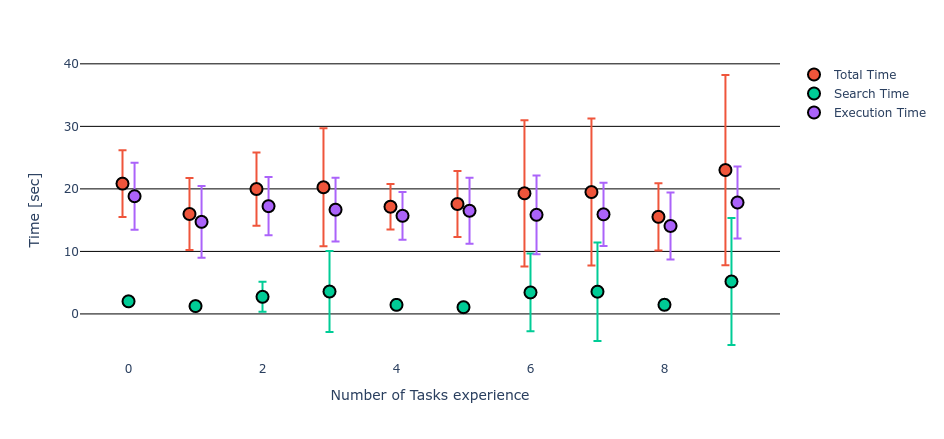
\includegraphics[width=0.9\textwidth]{figures/results/random_drive_kgraph}
    \caption{Search-, execution- and total time to complete a task. The horizontal axis indicates the number of task experience in a run. A run contains ten tasks, starting the run with an empty \ac{kgraph} that collects action feedback as the robot gains experience. The task contains three subtasks, in other words, the robot must drive to three target poses in order to complete a task. The vertical axis displays the mean and standart deviation of the search-, execution- and total time over ten runs, where the sum of seach- and execution time equals total time.}%
   \label{fig:rand_drive_times}
\end{figure}



Two available driving edge parameterisations are available, the \ac{MPC} and the \ac{MPPI} parameterisation that both use lti-drive-model to describe the point robot driving. In the following table it can be seen how many times the (\ac{MPC}, \textit{lti-drive-model}) parameterisation was selected versus the (\ac{MPPI}, \textit{lti-drive-model}) was selected.\bs

\begin{table}[H]
    \centering
    \begin{tabular}%
      {%
        >{\raggedright\arraybackslash}p{0.10\textwidth}
        >{\raggedright\arraybackslash}p{0.22\textwidth}
      |p{0.4cm}p{0.4cm}p{0.4cm}p{0.4cm}p{0.4cm}p{0.4cm}p{0.4cm}p{0.4cm}p{0.4cm}p{0.4cm}}
      \multicolumn{2}{c|}{Number of Tasks in experience} &0&1&2&3&4&5&6&7&8&9\\\toprule
      \multirow{4}{0.1\textwidth}{Without \ac{kgraph} suggestions} 
      &Number of \ac{MPC} parameterizations &14&14&12&12&17&16&17&19&16&11\\
      &Number of \ac{MPPI} parameterizations &19&19&21&21&17&17&18&14&17&22\\
      & \ac{MPC} selected for total drive actions [\%] &42&42&36&36&50&48&49&58&48&33\\
      & \ac{MPPI} selected for total drive actions [\%]&58&58&64&64&50&52&51&42&52&67\\\midrule
      \multirow{4}{0.1\textwidth}{With \ac{kgraph} suggestions} 
      &Number of \ac{MPC} parameterizations&22&33&34&33&33&33&33&34&33&32\\
      &Number of \ac{MPPI} parameterizations&11&0&0&0&0&0&0&0&0&0\\
      & \ac{MPC} selected in total drive actions [\%]&67&100&100&100&100&100&100&100&100&100\\
      & \ac{MPPI} selected in total drive actions [\%]&33&0&0&0&0&0&0&0&0&0\\
    \end{tabular}
    \caption{Influence of \ac{kgraph} suggestions in selecting the (\ac{MPC}, \textit{lti-drive-model}) parameterization versus selecting the (\ac{MPPI}, \textit{lti-drive-model} parameterization for drive actions.}%
    \label{table:rand_drive_mpc_vs_mppi}
\end{table}

\todo{compare pe with without kgraph}

What is not shown in the above figure is that the \ac{kgraph} over times prefers the \ac{MPC} controller over the \ac{MPPI} controller (both using the \textit{lti-model-1}) because of its lower average prediction error. The \ac{MPC} controller is a bit faster compared to the \ac{MPPI} controller thus the execution time decreases over time. The execution time is strongly correlated with the path length because driving to a target further away takes longer. It is thus only useful to investigate the trend that \Cref{fig:rand_drive_times} and not individual data points.\bs

\todo{Corrado: How are the suggestions built? Add a numerical example}
Then the same environments and tasks are solved 10 times without the \ac{kgraph} suggestions. The randomly generated tasks and environments are repeatable by fixing the seed. The fixed seed ensures that the randomly generated environments can be created multiple times, once to solve with \ac{kgraph} suggestions and once to solve without help from the \ac{kgraph}.\bs

\begin{figure}[H]
    \centering
    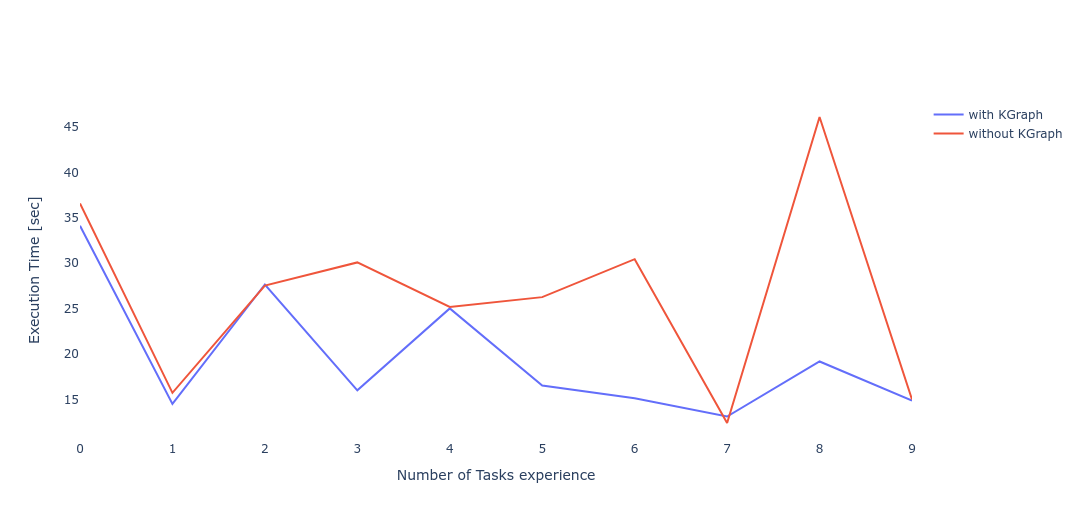
\includegraphics[width=0.9\textwidth]{figures/results/random_drive_with_without_kgraph}
    \caption{Execution times for driving toward target configurations with and without \ac{kgraph}.}%
    \label{fig:results_random_drive_task}
\end{figure}
\todo{Martijn: It is unclear what this image presents atm, and: If you repeat the experiment, will the graph look completely different?}

The figure above shows similar running times at the first few solved tasks. During these first tasks the \ac{kgraph}\todo{Corrado: How exactly } is filled with edge feedback, but the \ac{kgraph} has not gained enough feedback to suggest action parameterizations, this period can be referred to as the learning phase. After this learning phase, the \ac{kgraph} suggests the \ac{MPC} controller over the \ac{MPPI} controller, because of its relatively higher \textit{success factor} \todo{Corrado: You need to show these values otherwise it’s very vague}. The action suggestions improve overall execution time, note that selecting random controllers can result in equal execution time. In these cases, (4, 7 or 9 tasks in experience in \cref{fig:results_random_drive_task}) the randomly selected controllers all were \ac{MPC} controllers.\bs


\subsection{A Pushing Task}%
\label{subsec:rand_pushing}


\begin{figure}[H]
    \centering
    \begin{subfigure}{\textwidth}
    \centering
    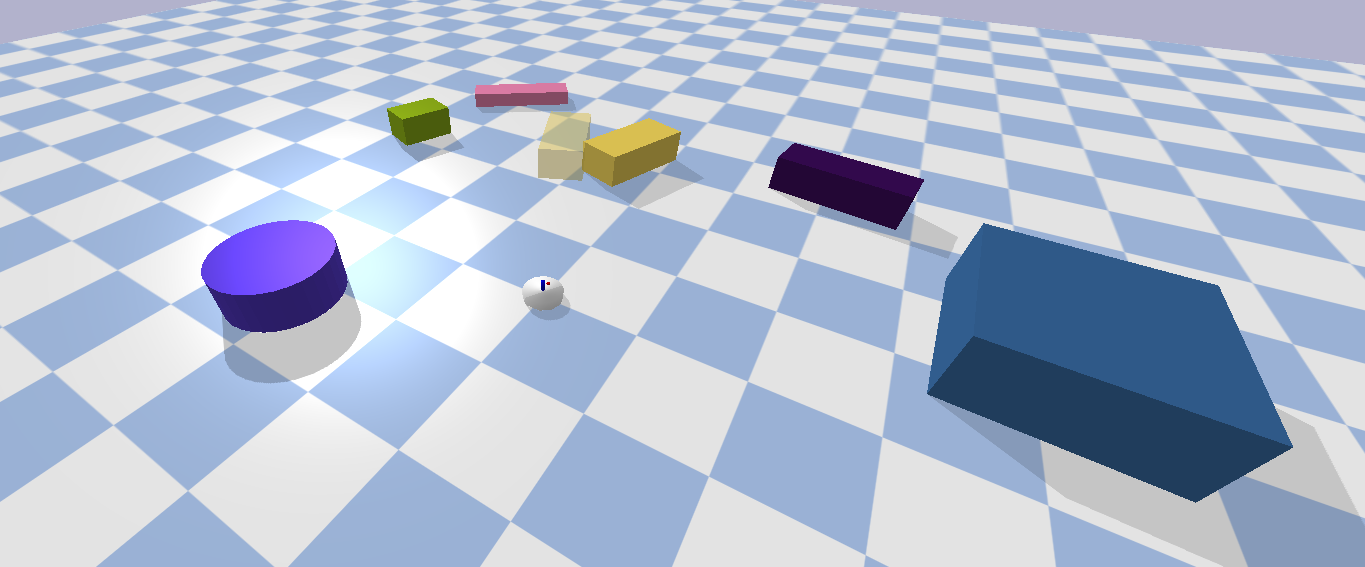
\includegraphics[width=0.9\textwidth]{figures/results/random_1}
    \end{subfigure}

    \vspace{0.2cm}
    \begin{subfigure}{\textwidth}
    \centering
    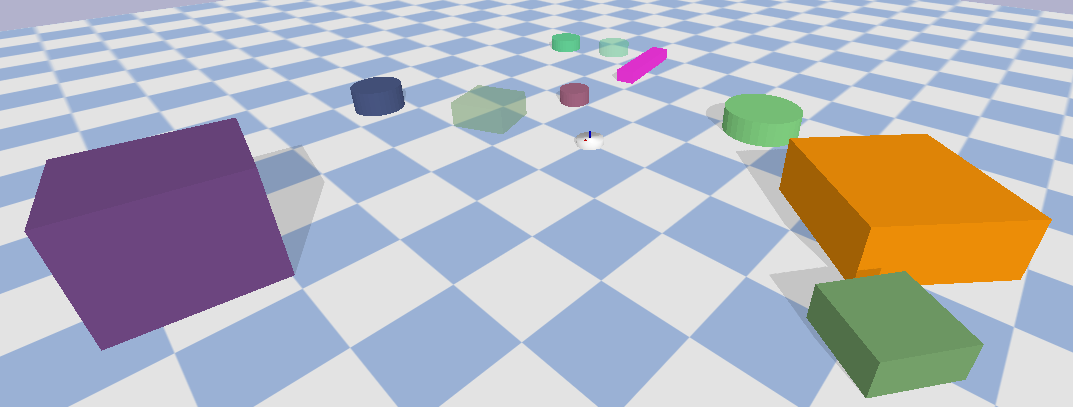
\includegraphics[width=0.9\textwidth]{figures/results/random_2}
    \end{subfigure}
    \caption{Two random environments with 2 target ghost configurations for the task containing 2 subtasks.}%
    \label{fig:random_environnment}
\end{figure}


Now the \ac{halgorithm} is tasked with pushing a single object toward a target configuration. Except for the number of subtasks all parameters that determine the random environment will remain as previously set for the random driving task.\bs

\begin{figure}[H]
    \centering
    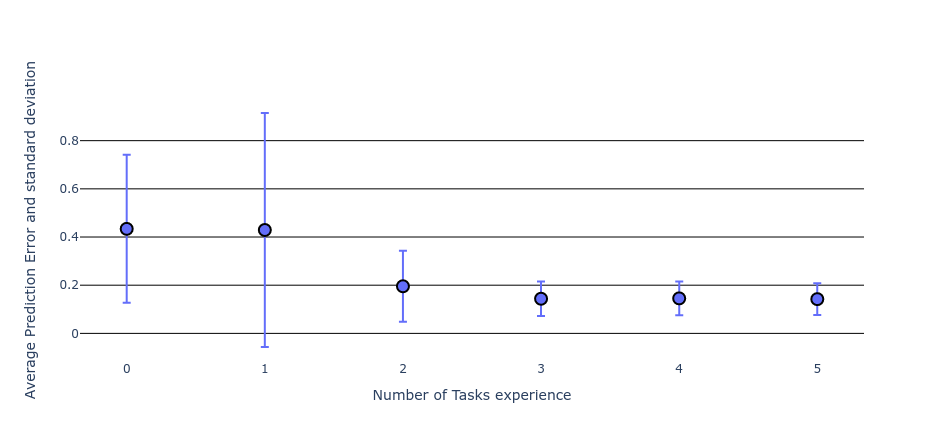
\includegraphics[width=0.9\textwidth]{figures/results/random_pe_push_kgraph}
    \caption{Average Prediction Error and Standard Deviation for action edges during a pushing task.}%
    \label{fig:rand_push_full_pred}
\end{figure}

\begin{figure}[H]
    \centering
    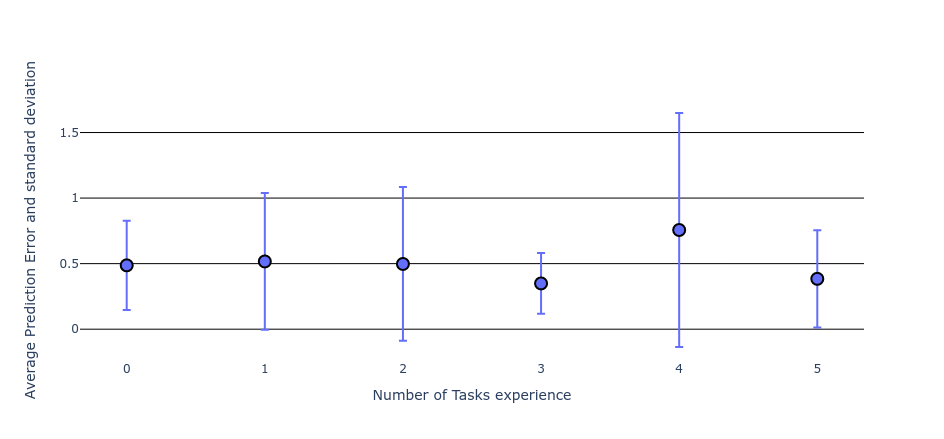
\includegraphics[width=0.9\textwidth]{figures/results/random_pe_push_no_kgraph}
    \caption{wanna do TODO something with this?? maybe add to above plot}%
    \label{fig:rand_push_full_pr}
\end{figure}

\todo{Martijn: averaged over how many experiments? related to that 1.5 and 2 }
The \ac{MPPI} controller with \textit{nonlinear-push-model-1} has an average \ac{PE} between 1.5 and 2 and can be seen in the figure above as the most left data point in the prediction error plot. The same controller with \textit{nonlinear-push-model-2} has an average lower \ac{PE} between 0.4 and 0.6 and can be seen in the following data points (1, 2, 3 and 4). The \textit{success factor} \todo{Corrado: unclear how suc factor is defines, How exactly… put a reference to the formula number} is calculated based on the average prediction error so it is expected that the \ac{kgraph} suggests the controller with the lower prediction error. It is expected that the \ac{PE} goes down, which is exactly what \Cref{fig:rand_push_full_pred} shows. The \ac{halgorithm} tests both edge parameterisations to conclude that the \ac{MPPI} controller and \textit{nonlinear-push-model-2} is the better of the two.

\begin{figure}[H]
    \centering
    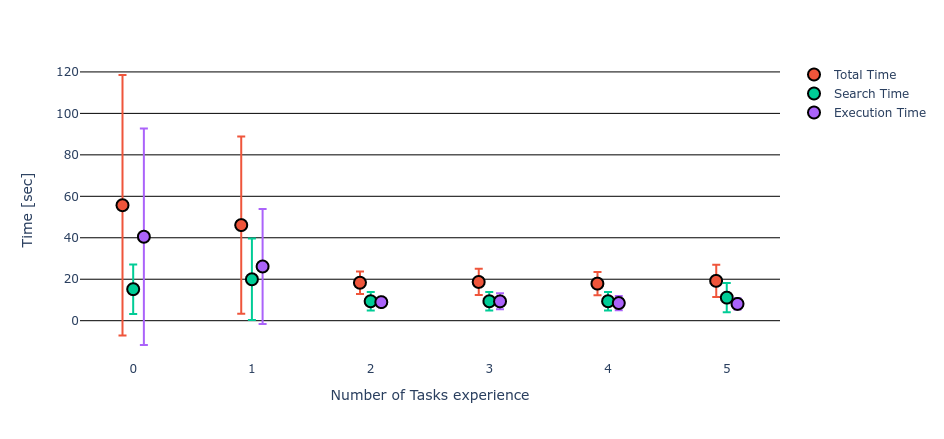
\includegraphics[width=0.9\textwidth]{figures/results/random_push_kgraph}
    \caption{Planning times for pushing an object toward the target a configuration.}%
    \label{fig:random_push_all_times}
\end{figure}

\todo{Corrado: A plot should be self contained, but there is no mention to the models used and there is no way to see that for myself from the graph }

The \ac{MPPI} controller with \textit{nonlinear-push-model-2} does not only have a lower \ac{PE} but is also faster compared to the \ac{MPPI} controller combined with \textit{nonlinear-push-model-1}. Execution time for driving toward the object and pushing that object to its target location takes around 15 seconds, with a search time to find that hypothesis being between 10 to 15 seconds. The result is that task execution time lowers, bear in mind that this result has to be taken with a grain of salt because the execution time is correlated with the path length (how far the object is from the robot, and how far should the object be pushed). It is better to look at the figure below that displays the execution time of both solving the same task with help of the \ac{kgraph} and without its help.

\begin{figure}[H]
    \centering
    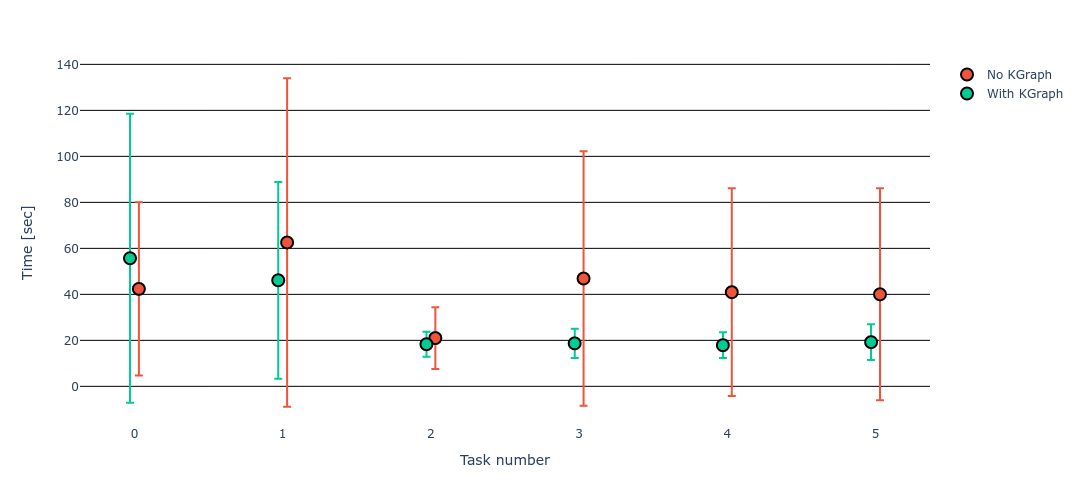
\includegraphics[width=0.9\textwidth]{figures/results/random_push_with_without_kgraph}
    \caption{Execution times for pushing an object to target configurations with and without \ac{kgraph}.}%
    \label{fig:random_push_with_without_kgraph}
\end{figure}



The \ac{kgraph} suggestion work in favour of the execution time as can be seen in the \Cref{fig:random_push_with_without_kgraph}. Noticable is that a random selection by pure change selects the best choice of the controller as can be seen in 2 tasks of experience in the figure above.

\begin{table}[H]
    \centering
    \begin{tabular}%
      {
        >{\raggedright\arraybackslash}p{0.10\textwidth}
        >{\raggedright\arraybackslash}p{0.35\textwidth}
      |p{0.4cm}p{0.4cm}p{0.4cm}p{0.4cm}p{0.4cm}p{0.4cm}}
      \multicolumn{2}{c|}{Number of Tasks in experience} &0&1&2&3&4&5\\\toprule
      \multirow{4}{0.1\textwidth}{Without \ac{kgraph} suggestions} 
      &Number of \textit{nonlinear-push-model-1} parameterizations&4&3&7&5&4&5\\
      &Number of \textit{nonlinear-push-model-2} parameterizations&5&5&3&5&6&4\\
      & \textit{nonlinear-push-model-1} selected in total push actions [\%]&44&38&70&50&40&56\\
      & \textit{nonlinear-push-model-2} selected in total push actions [\%]&56&62&30&50&60&44\\\midrule
      \multirow{4}{0.1\textwidth}{With \ac{kgraph} suggestions} 
      &Number of \textit{nonlinear-push-model-1} parameterizations&4&5&8&10&10&10\\
      &Number of \textit{nonlinear-push-model-2} parameterizations&5&4&2&0&0&0\\
      & \textit{nonlinear-push-model-1} selected in total push actions [\%]&44&56&80&100&100&100\\
      & \textit{nonlinear-push-model-2} selected in total push actions [\%]&56&44&20&0&0&0\\
    \end{tabular}
    \caption{Influence of \ac{kgraph} suggestions in selecting the (\ac{MPPI}, \textit{nonlinear-push-model-1}) parameterization versus selecting the (\ac{MPPI}, \textit{nonlinear-push-model-2}) parameterization for push actions.}%
    \label{table:rand_push_model1_vs_model2}
\end{table}

\todo{Corrado: The numbers above do not always count up to 10, because not all tasks are succesfully completed. how to account for that?}

\section{Comparison with State-of-the-Art}%
\label{sec:compare_with_related_papers}
\todo{Corrado: This should be structured better, it is an important part}

In the introduction \Cref{table:sota_and_3_topics} was presented. A table that mainly shows which subset of the 3 main topics are included in which scientific paper. The 3 topics are learning system models, the \ac{NAMO} problem and nonprehesile pushing. The table is presented again with the addition of the main testing method that is used by the state-of-the-art paper.

\noindent
\begin{table}[H]
  \centering
  \rowcolors{2}{white}{myEvenLighterColor}
  \begin{tabular}
  {>{\raggedright\arraybackslash}P{1.8cm}%
    >{\raggedleft\arraybackslash}P{1.4cm}%
    >{\raggedright\arraybackslash}P{1.2cm}%
    >{\raggedright\arraybackslash}P{1.2cm}%
    >{\raggedright\arraybackslash}P{1.2cm}%
    >{\raggedright\arraybackslash}P{1.6cm}
    >{\raggedright\arraybackslash}P{3.8cm}
  }
  Author & Citation & Learns\newline object\newline dynamics & \ac{NAMO} & Specify object target positions & Object\newline Manipu- lation & test metric\\
  \citeauthor{ellis_navigation_2022} &\cite{ellis_navigation_2022} & \cmark& \cmark& \xmark& pushing & \underline{success rate}\\
\citeauthor{sabbaghnovin_model_2021} &\cite{sabbaghnovin_model_2021} & \cmark& \xmark& \cmark& grasp-push grasp-pull & success rate, \underline{execution time} \underline{prediction error}, final position error \\
\citeauthor{scholz_navigation_2016} &\cite{scholz_navigation_2016} & \cmark& \cmark& \xmark& graph-push grasp-pull & runtime, planning time, \underline{number of calls to planner} number of calls to update model\\
\citeauthor{vega-brown_asymptotically_2020} &\cite{vega-brown_asymptotically_2020} & \xmark& \cmark& \cmark& gripping & \underline{computation time}\\
\citeauthor{wang_affordancebased_2020} &\cite{wang_affordancebased_2020} & \cmark& \cmark& \xmark& pushing & \underline{computation and} \underline{execution time}\\
    Groote & proposed solution &  \xmark/\cmark& \cmark& \cmark& pushing & see \Cref{table:proposed_method_metrics}\\
  \end{tabular}
  \caption{Overview of recent state-of-the-art papers that include a subset of the 3 topics (learning system models, \ac{NAMO}, and nonprehensile pushing). The \textit{grasp-push} and \textit{grasp-pull} refer to prehensile push and pull manipulation, \textit{gripped} refers to fully gripping and lifting objects for manipulation, \textit{pushing} refers to nonprehensile push manipulation. The test metric indicates the testing method used by the paper, where the underlined metric is used to compare against the proposed framework.}%
\label{table:sota_vs_results_proposed method}
\end{table}
\todo{update this table with the table from waaaaay above}

\paragraph{Comparing Success Rate}
\citeauthor{ellis_navigation_2022} claims to push with a success rate \todo{Corrado: perhaps eleborate on that 100 percent, how does ellis define that?} of a 100\%~\cite{ellis_navigation_2022}. The test environment that \citeauthor{ellis_navigation_2022} has used is very similar to the random pushing task discussed in \Cref{sec:randomisation}. For both the random driving task and the random pushing task the success rate is 100\%. Meaning that every driving or pushing subtask was successfully completed. It is even so that for the result of the random push task (displayed in \Cref{fig:rand_push_full_pred,fig:random_push_all_times,fig:random_push_with_without_kgraph}) the number of hypotheses is equal to the number of subtasks \todo{Corrado: How do I see this? unclear to tthe reader}. Meaning that every subtask is completed by the first hypothesis generated. Both similar experiments from \citeauthor{ellis_navigation_2022} and this thesis have a 100\% success rate for similar
, allowing us to conclude that the results are comparable.

\paragraph{Comparing Computation and Execution Time}
Three state-of-the-art papers that use computation and execution time as the testing metrics are compared to the proposed framework. To accomplish a fair comparison the environments that have been used in the \todo{Corrado: Where do I see this?} citations are rebuilt in the pybullet software. The results are then directly compared to conclude that the proposed framework is as good as or even better in terms of computation time and execution time for similar tasks.\bs

\citeauthor{wang_affordancebased_2020}
\todo{Corrado: Comparison with wang

In this experiment we compare against Wang. The goal is to reach a target location,but the robotis reuiredto free the path first. The visialized in fig.

caption

Experiment from wang, reproduction of the experiment

We run the experiment 10 times with different initial positions and goals.The results are reported in table.. }
drives toward a target configuration that is blocked by a chair. \todo{Corrado: By Wang or you?} The task is performed 3 times where the robot may remember its interactions with the chair from previous runs. The task is successfully completed all three times with a total time of 200 seconds for the first run to 180 seconds for the third run. Execution time increased from 70 to 85 seconds during these runs \todo{Corrado: Why?}. Even with increasing execution times, the solution is found faster because the experience from previous runs could be used that lowered search time~\cite{wang_affordancebased_2020}. To compare against these results the environment is recreated in the pybullet software \todo{Corrado: Show the recreated env then!}. The proposed framework was run only once, during this run it classified a wall object as unmovable, and the pushable box object with dimensions equal to that of the chair was classified as movable and moved out of the way. Overall execution time was 45 seconds whilst computation time took 65 seconds. The proposed framework successfully completed this similar task whilst having a lower computation and execution time. This allows concluding that the proposed framework improves upon the paper from \citeauthor{wang_affordancebased_2020} with a decent margin.\bs
\todo{Corrado: Put a screenshot side by side of your environment and Wang one}

\citeauthor{vega-brown_asymptotically_2020} has a task that pushes two boxes into a goal region. It takes around 300 seconds to return a hypothesis~\cite{vega-brown_asymptotically_2020}. \todo{Corrado: What do you mean? for the next sentce}Both pushing tasks can be compared with two separate pushing tasks from the random push environment. By doubling the time to push a single object to its target configuration, $2 \cdot 30 = 60$ seconds both tasks could be compared. However, the point of \citeauthor{vega-brown_asymptotically_2020} paper is that a global minimal task is sought. The proposed framework randomly selects a subtask and tries to complete it to then move to the next randomly selected subtask. A global minimum is thus not sought and both papers can therefore not be compared properly.\todo{Corrado: Then why including it in the comparison?}\bs

\citeauthor{sabbaghnovin_model_2021} grasp-pushes and grasp-pulls a walker object to two new target configurations~\cite{sabbaghnovin_model_2021}. The task is mimicked by pushing a box object of equal dimensions to the same target configurations. Compared to \citeauthor{sabbaghnovin_model_2021} average of 125 and 160 seconds to complete task 1 and task 2 the proposed framework takes an average of only 27 and 33 seconds respectively (10 seconds computation time) to complete similar tasks. The decrease in total time allows to conclude that the proposed frameworks improve upon the method proposed by~\citeauthor{sabbaghnovin_model_2021}.\bs \todo{Corrado: So your pushing controllers are performin better than prehensile manipulation? amazing, but doub}

\paragraph{Comparing Prediction Error}
\citeauthor{sabbaghnovin_model_2021} displays the final position errors for a selection of objects which range from 0.05 to 0.6 meters. A success threshold is set to 0.1 meters, which determines that the object is at its target location~\cite{sabbaghnovin_model_2021}. The success threshold in this thesis is set to a staggering 0.9 meters,\todo{Corrado: But then how can you compare success rate if you have different metrics for success?} thus it is concluded an object has reached its target position, whilst it is still 0.9 meters from its target configurations. This thesis does not try to reach optimal control, it tries to select the best controller in the available set of controllers. If the same controller from \citeauthor{sabbaghnovin_model_2021} would be available, then similar final position errors would be obtained. It can be concluded that the prediction error \todo{Corrado: Not position errro?}of the proposed framework is worse compared to this state-of-the-art. The reason is that the proposed framework focuses on improving the control selection and action sequences over time, and not on lowering final prediction errors.\bs

% \paragraph{Comparing Number of Replanning times}
% \todo[inline]{\cite{scholz_navigation_2016}}
